%%%%%%%%%%%%%%%%%%%%%%%%%%%%%%%%%%%%%%%%%
% Vertical Line Title Page 
% LaTeX Template
% Version 1.0 (27/12/12)
%
% This template has been downloaded from:
% http://www.LaTeXTemplates.com
%
% Original author:
% Peter Wilson (herries.press@earthlink.net)
%
% License:
% CC BY-NC-SA 3.0 (http://creativecommons.org/licenses/by-nc-sa/3.0/)
% 
% Instructions for using this template:
% This title page compiles as is. If you wish to include this title page in 
% another document, you will need to copy everything before 
% \begin{document} into the preamble of your document. The title page is
% then included using \titleGM within your document.
%
%%%%%%%%%%%%%%%%%%%%%%%%%%%%%%%%%%%%%%%%%

%----------------------------------------------------------------------------------------
%	PACKAGES AND OTHER DOCUMENT CONFIGURATIONS
%----------------------------------------------------------------------------------------

\documentclass{article} 
\usepackage{titlesec}
\usepackage[utf8]{inputenc}
\usepackage{tocloft}
\usepackage[margin=1in]{geometry}
\usepackage{graphicx}
\usepackage{enumitem}
\renewcommand{\cftsecleader}{\cftdotfill{\cftdotsep}}

\newcommand*{\plogo}{} % Generic publisher logo

\usepackage{float,array}
\usepackage{chngcntr}
\counterwithin{figure}{section}
\usepackage{booktabs} % To thicken table lines

%----------------------------------------------------------------------------------------
%	TITLE PAGE
%----------------------------------------------------------------------------------------

\newcommand*{\titleGM}{\begingroup % Create the command for including the title page in the document
\hbox{ % Horizontal box
\hspace*{0.2\textwidth} % Whitespace to the left of the title page
\rule{1pt}{\textheight} % Vertical line
\hspace*{0.05\textwidth} % Whitespace between the vertical line and title page text
\parbox[b]{0.75\textwidth}{ % Paragraph box which restricts text to less than the width of the page

{\noindent\Large\bfseries Software Design Document \\[0.5\baselineskip] for Smart Fridge Kitchen Assistant}\\[2\baselineskip] % Title
{\tiny \textit{Prepared by Sai Sivva, Ahmed Humayun, and Joshua Wilson on behalf of the Smart Fridge Team}}\\[4\baselineskip] % Tagline or further description
{\Large \textsc{joshua wilson\\sai sivva\\ahmed humayun\\shu yang\\zhen li}} % Author name

\vspace{0.5\textheight} % Whitespace between the title block and the publisher
{\noindent CSC 532: Software Engineering \plogo}\\[\baselineskip] % Publisher and logo
}}
\endgroup}

\setcounter{tocdepth}{2}
%----------------------------------------------------------------------------------------
%	BLANK DOCUMENT
%----------------------------------------------------------------------------------------
\titleformat{\subsubsection}[runin]
{\normalfont\normalsize\bfseries}{\thesubsubsection}{1em}{}
\begin{document}

\pagestyle{empty} % Removes page numbers

\titleGM % This command includes the title page
\tableofcontents

\section*{Revision History}
{\ttfamily\begin{center}
		\begin{tabular*}{\textwidth}{ m{4em} m{5em} m{25em} m{4em}  }		
			\toprule			
			Rev.\# & Date & Nature of Revision & Version \\
			\bottomrule
			\toprule
			1 & 10.30.2016 & ORIGINAL VERSION & 1.0\\
			
			\hline		
		\end{tabular*}
	\end{center}
}
\pagebreak

\section{Introduction}
The main purpose of the Software Requirement Specifications (SRS) is to provide information about what is to be expected of the Smart Fridge Kitchen Assistant upon completion. This document specifies all the functional and non-functional requirements of the software being developed, and explains all the entities involved in the development of the software.

\subsection{Purpose}
\subsubsection{Vision Statement} At the core, the system is a user interface for kitchen inventory management. However, it will help the user to maintain their personalized nutrition plans, and provide feedback to reduce energy and food waste. While there do exist other fully contained smart fridges with integrated touch screen panels, the cost of these are prohibitively expensive for most people. This project aims to create an inexpensive product which one may use with ones current ``dumb" refrigerator. The project may be used as a standalone system or may be integrated with other smart house applications. 
\subsubsection{Scope} The scope of this project is to refine the existing Smart Fridge Project. This includes creating a user interface for using for a touch screen platform, implementing a customizable nutrition plan for the user, broadening the project to include several inventories, and allowing for a bulk fridge update using information from receipts. Additionally, the product will allow for integration with the Pillar smart house project.


\subsection{Document Conventions}
This document follows MLA Format which suggests to use bold-faced text to emphasize section and sub-section headings. Underlining is to point out words in the glossary and italicized text is
used to label and recognize diagrams.

\subsection{Intended Audience and Reading Suggestions}
This document is intended to be read by the developers, testers, project manager, system architect, and analysts of the Smart Fridge Team. 

\subsection{References}
Unless otherwise noted, all figures may be found at the end of the document.

\section{Overall Description}
The Smart Fridge Kitchen Assistant is a refinement of an existing Smart Fridge product. The software is a Java web application to be accessed on an apache server run by a Raspberry Pi 3 with attached touchscreen an camera  modules. 

\subsection{Product Perspective} The smart fridge inventory management system helps to keep track food items and can generate shopping list based on personalized nutrition preferences, save energy by suggesting temperature based on inventory, and manage the trash generated due to expired products.

\subsection{Product Functions} The main function of this project is to improve the customer experience by improving the user interface and adding functionality. The key features are as follows:
\begin{enumerate}
	\item Uses information available on grocery receipts to determine each of the UPCs from the groceries that the user has purchased. The system will then communicate with a product database through the Nutritionix\texttrademark API to determine the nutritional information about the product. The product, along with the nutritional information is the entered into the database automatically and an approximate expiration date is set for the item.  
	\item Allows for touch querying and updating through a newly designed interface. This interface will also display the contents of the refrigerator via icons representing each food item. 
	\item Generates personalized shopping list based on nutritional needs and expiration of current food items. 
	\item Integrates a waste and energy model. Waste from spoiled is approximated and shown to the user. This feedback will allow them to reduce spoilage in the future. Additionally, a  temperature is suggested from the contents of the refrigerator. This may either be integrated with an existing fridge temperature adjustment system, or the user can manually adjust the temperature of their fridge. 
	\item Integration with the Pillar smart home system to allow Pillar to access the Smart Fridge database and make adjustments as needed. 
\end{enumerate}


\subsection{User Classes and Characteristics}

The target users of this system are middle to low income users who wish to keep track of their food consumption and waste. After creating an account, users specify their nutritional needs (e.g. weight loss, high protein diets, vegan) based on which a nutrition plan is constructed. Additionally, the user may, with the aid of the software, create weekly meal plans from which shopping lists are created.  

\subsection{Operating Environment}
The software is developed to run as a web application on a LAMP server hosted by a Raspberry Pi 3, which uses Raspbian (a Debian-based operating system). In principle, any computer or mobile device on the same network as the Raspberry Pi will be able to access the server through an Internet browser. 

\subsection{Design and Implementation Constraints}
The Raspberry Pi 3 (RPi3) has Model B Quad-Core 1.2 GHz 1 GB RAM, On-board WiFi and Bluetooth Connectivity.

\subsection{User Documentation}
Dr. Box and the previous team have already prepared the user document for the previous version. We intend to add details of the new specifications to that document and we will present it to the user.

\subsection{Assumptions and Dependencies}
It is assumed that the receipts contain QR codes which allow for the system to obtain the UPC of all products purchased by the user upon scanning. Each user must create a user ID, and all food additions and consumptions from the fridge are properly logged. 

\section{External Interface Requirements}

\subsection{User Interfaces}
The main aim is to provide a bulk update feature along with personalized nutrition plans, shopping lists, and an overhauled user interface. Reference Figure~\ref{GUI1} and Figure~\ref{GUI2} for the current user interface. 
\begin{figure}[p]
	\centering
	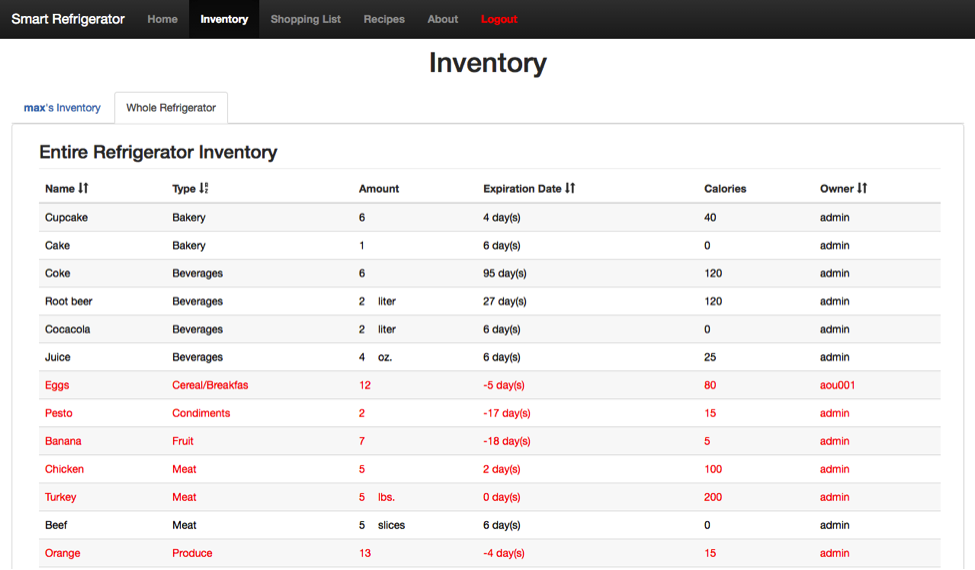
\includegraphics[width=\textwidth]{gui.png}
	\caption{Inventory interface from previous project showing the inventory}
	\label{GUI1}
\end{figure}
\begin{figure}[p]
	\centering
	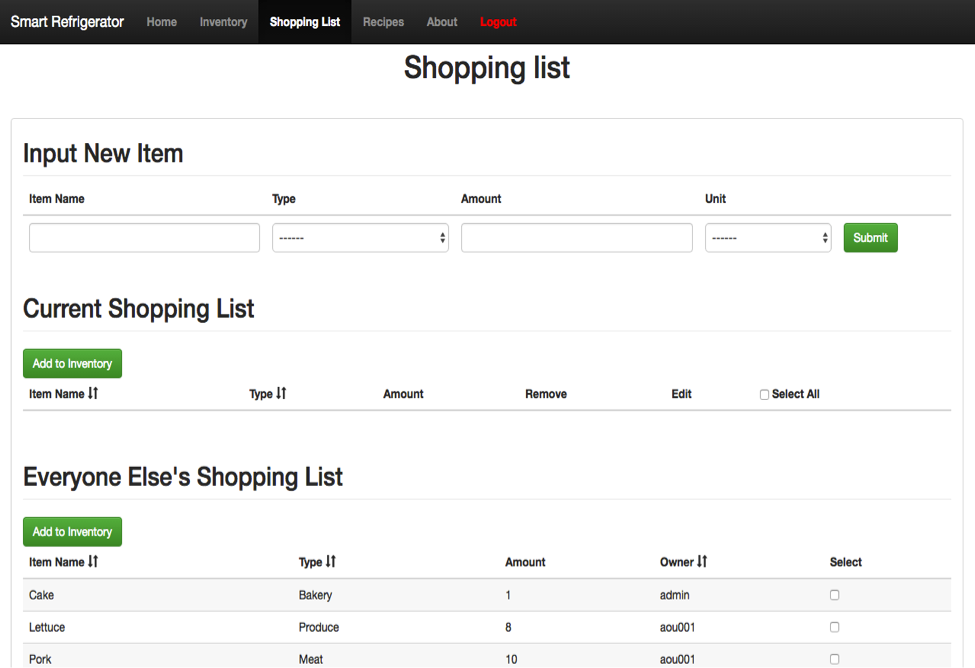
\includegraphics[width=\textwidth]{gui1.png}
	\caption{Shopping list interface from previous project showing the inventory}
	\label{GUI2}
\end{figure}
\subsection{Hardware Interfaces} The product uses the a Raspberry Pi Camera module to scan a receipt for a QR code. The Raspberry Pi Touchscreen module is used for the touchscreen GUI. 

\subsection{Software Interfaces} The product is a web application to be included in an Apache server which is developed to run on a Raspberry Pi running the Raspbian Jessie operating system. In principle, however, this may be run from any computer with the appropriate server, camera, and touch screen configuration. 

\subsection{Communications Interfaces} The product is designed to interface with use the Nutritionix API to interface with their database. Additionally, the product will communicate with the Pillar through yet-to-be-developed interface. 

\section{System Features}
	\subsection{Registration}
	\subsubsection{Goal:} To register the user into the database and to gather health and dietary information. 
	\subsubsection{Input:} user ID, password, health and dietary information
	\subsubsection{Output:} User registration successful, added user to database
	\subsubsection{Main Scenario:} To register the user into the database and to gather health and dietary information. 
	\subsubsection{Pre-Condition:} Registration screen displayed
	\subsubsection{Steps:} 
\begin{enumerate}\setlength\itemsep{-1em}
	\item User selects ``register'' from screen\\
	\item User specifies user ID, password\\
	\item and health and dietary information on screen. 
\end{enumerate}
	\subsubsection{Post-Condition:} User information stored into database
	\subsubsection{Representation:} See Figure~\thesubsection
	\begin{figure}[p]
	\centering
	
\includegraphics[width=\textwidth]{registration.png}
	\caption{Registration}
	\end{figure}
	\subsection{Login}
		\subsubsection{Goal:} To allow the user to login to the web application  
		\subsubsection{Input:} user ID, password
		\subsubsection{Output:} user credentials verified
		\subsubsection{Main Scenario:} User is authenticated and brought to home page
		\subsubsection{Pre-Condition:} Login screen is displayed
		\subsubsection{Steps:} 
		\begin{enumerate}
			\item User inputs credentials into login screen
			\item Credentials are checked against user database
			\item User is verified
		\end{enumerate}
		\subsubsection{Post-Condition:} Homepage is displayed
		\subsubsection{Representation:} See Figure~\thesubsection
		\begin{figure}[p]
			\centering
			
\includegraphics[width=\textwidth]{login.png}
			\caption{Login}
		\end{figure}
		
	\subsection{Bulk Update}
	
		\subsubsection{Goal:} Allows user to update fridge with information from receipt
		\subsubsection{Input:} Photograph of receipt
		\subsubsection{Output:} Item and nutritional information input into database
		\subsubsection{Main Scenario:} User needs to update large quantify of items which were recently purchased
		\subsubsection{Pre-Condition:} User is logged in an camera module is activated
		\subsubsection{Steps:} 
		\begin{enumerate}
			\item User holds receipt up to camera
			\item QR code from receipt is scanned
			\item From QR code, UPC information is gathered
			\item UPC information is used with Nutritionix API to determine nutritional information
			\item Item nutritional information and nutritional information entered into inventory database
		\end{enumerate}
		\subsubsection{Post-Condition:} Inventory screen is displayed
		\subsubsection{Representation:} See Figure~\thesubsection
		\begin{figure}[p]
			\centering
			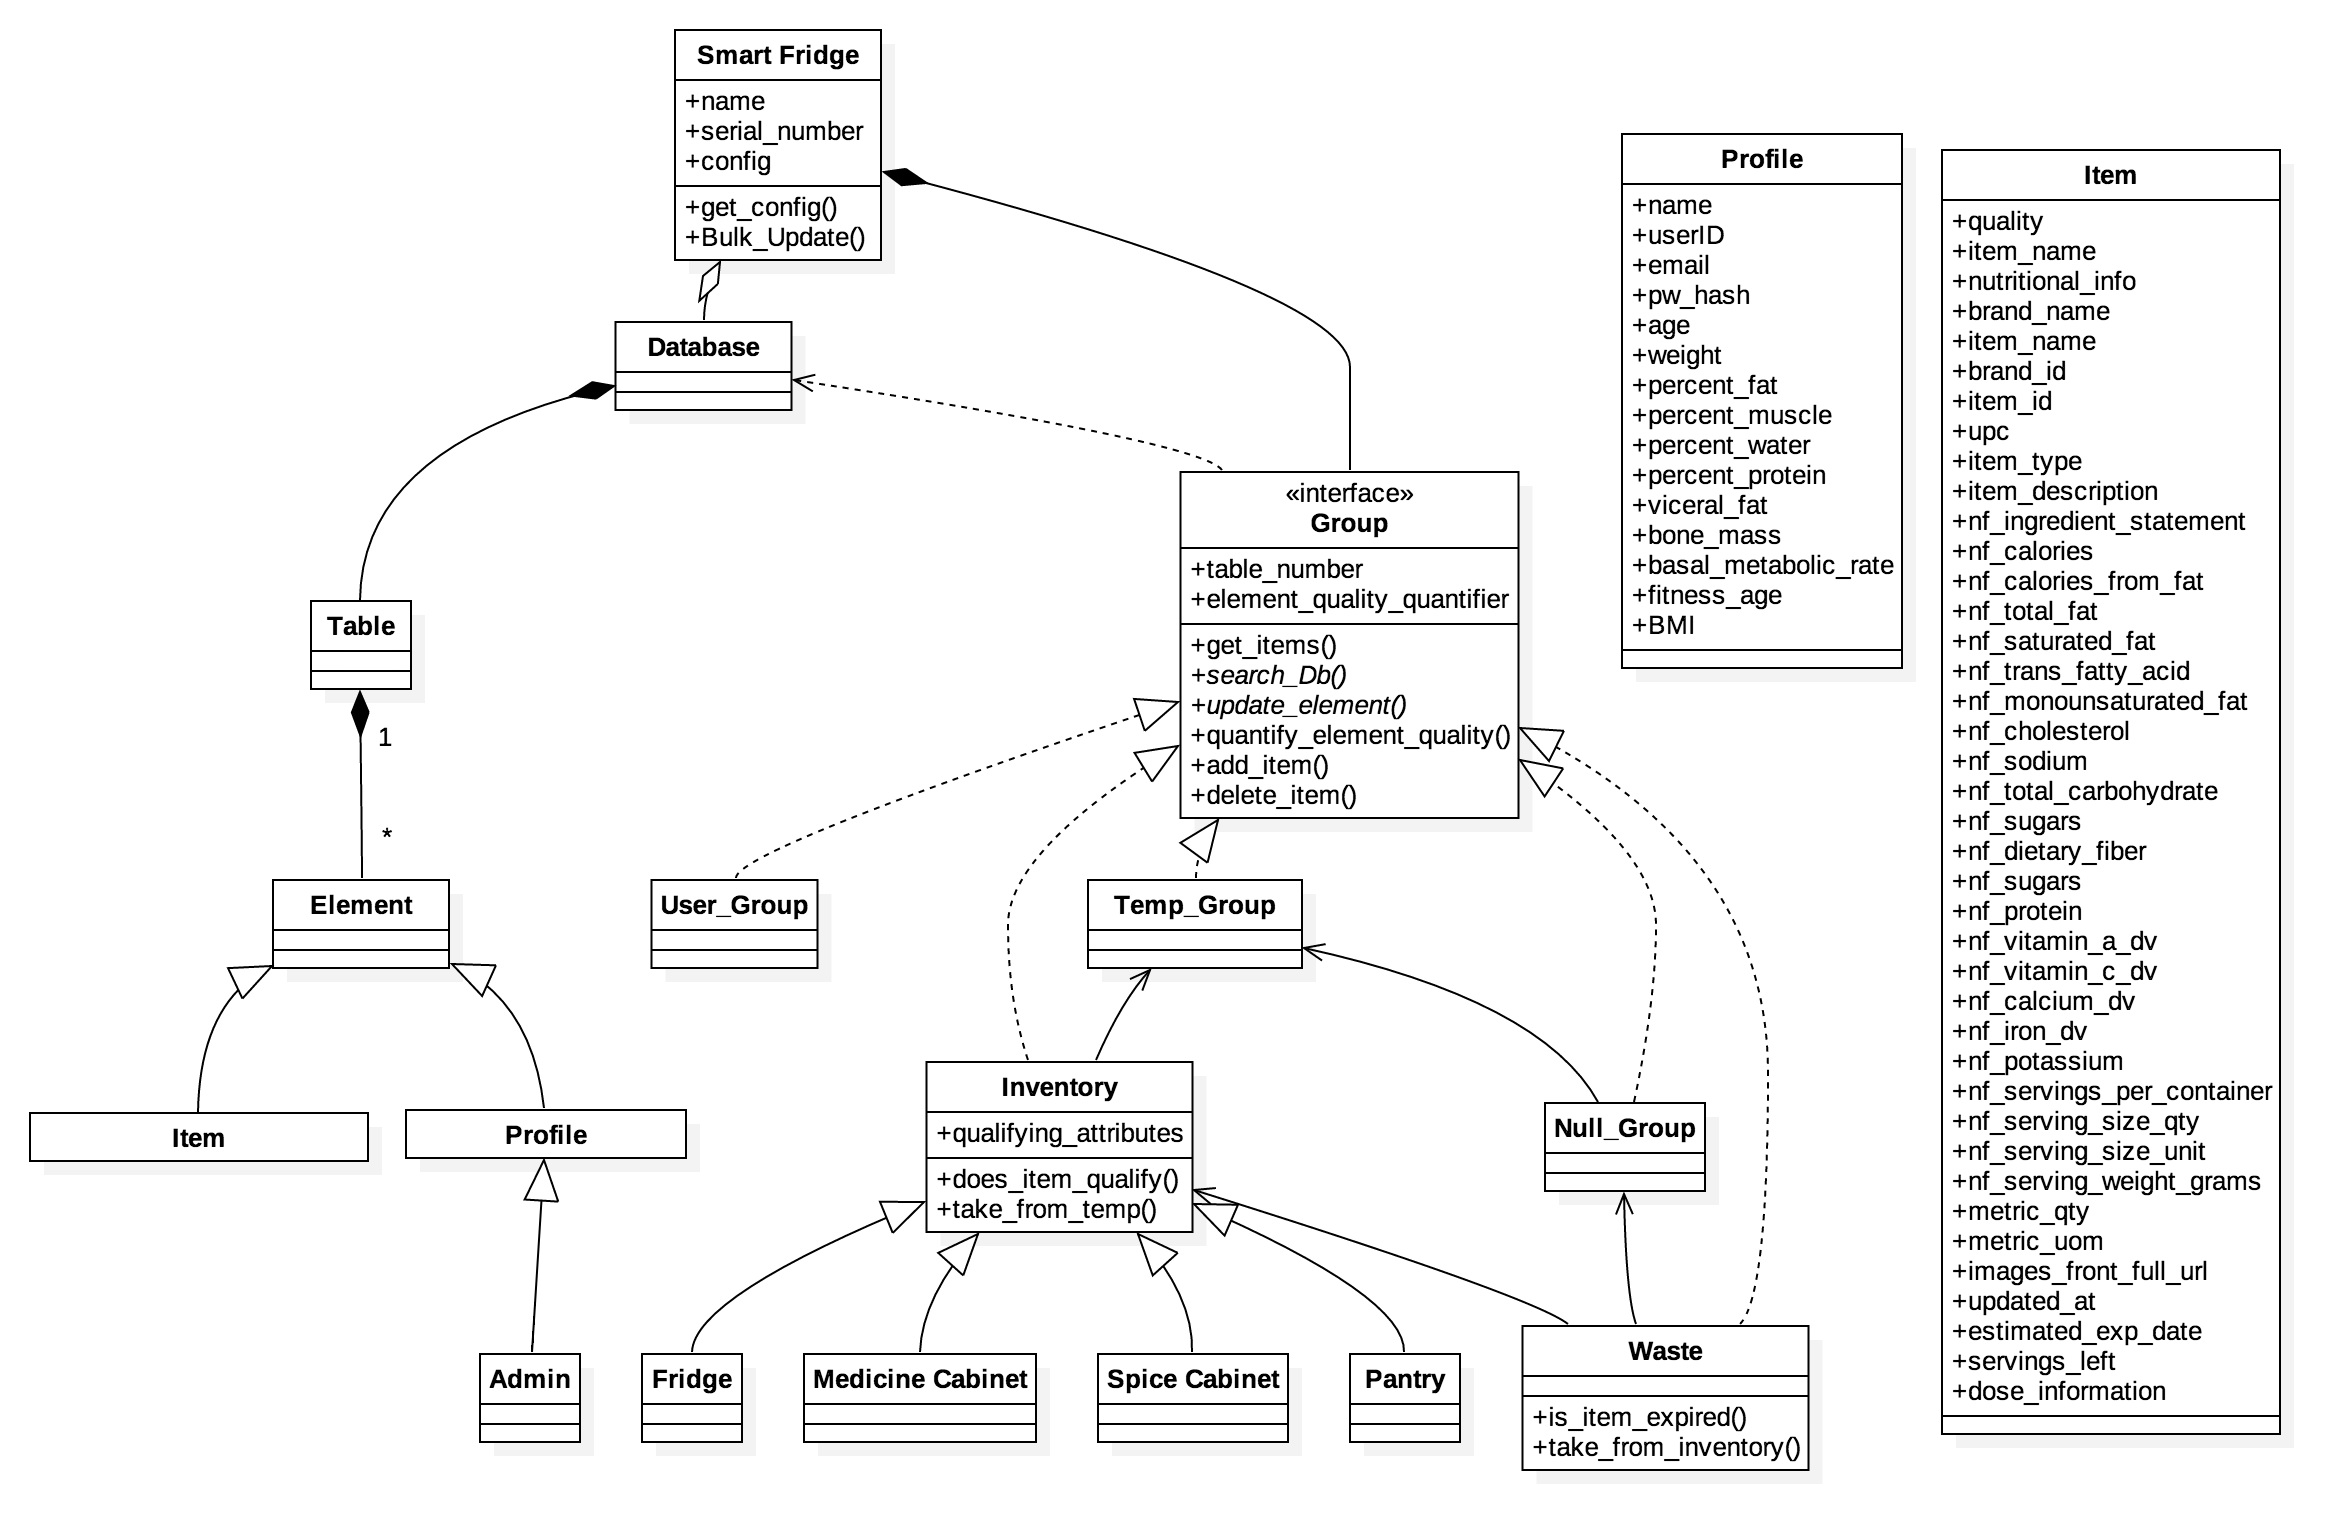
\includegraphics[width=\textwidth]{bulkupdate.png}
			\caption{Bulk Update}
		\end{figure}
	
	\subsection{Display Fridge Contents and Single Item Update}
		\subsubsection{Goal:} To allow the user to know the contents of the fridge without opening the fridge
		\subsubsection{Input:} User request to see contents
		\subsubsection{Output:} Display contents on screen, updated database
		\subsubsection{Main Scenario:} User wishes to see the smart fridge inventory and/or update the contents 
		\subsubsection{Pre-Condition:} User is logged in
		\subsubsection{Steps:} 
		\begin{enumerate}
			\item User uses touch screen to request contents of fridge 
			\item Query Inventory Database for contents
			\item Display Inventory Icons on screen
			\item User touches icon
			\item Display number of items and nutritional information
			\item User edits item information
		\end{enumerate}
		\subsubsection{Post-Condition:} Display Inventory Page
		\subsubsection{Representation:} See Figure~\thesubsection
		\begin{figure}[p]
			\centering
			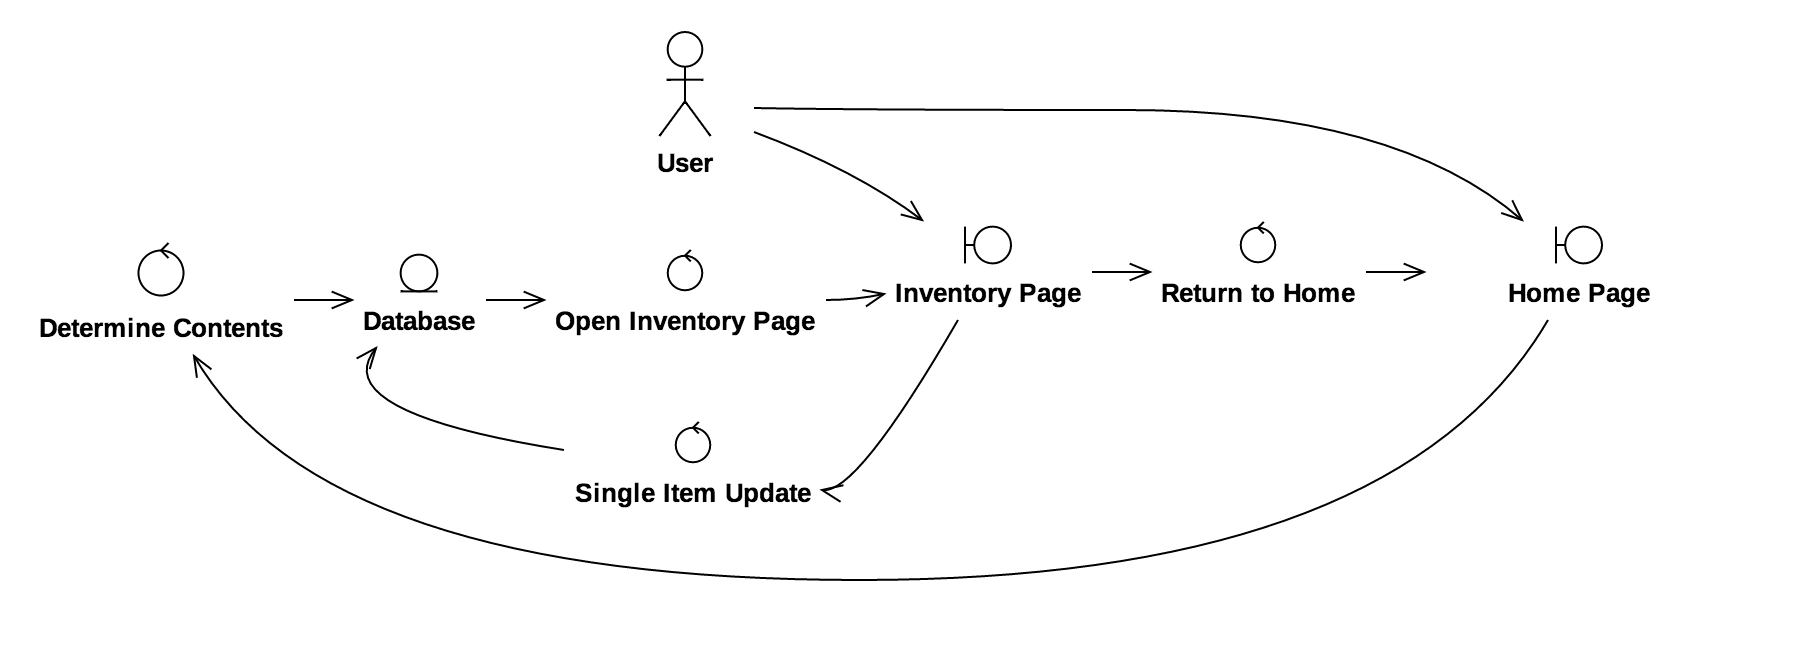
\includegraphics[width=\textwidth]{displayinv.png}
			\caption{Display Fridge Contents and Single Item Update}
		\end{figure}
	\subsection{Manual Update}
		\subsubsection{Goal:} Allows the user to manually enter and edit items in database as spreadsheet
		\subsubsection{Input:} Item and Nutritional information
		\subsubsection{Output:} Database updated
		\subsubsection{Main Scenario:} User needs to enter items without receipt which are not already in the fridge. 
		\subsubsection{Pre-Condition:} User is logged in and on main page
		\subsubsection{Steps:} 
		\begin{enumerate}
			\item User request inventory spreadsheet screen
			\item User adds or changes database entries
			\item User confirms changes
			\item Home screen displayed
		\end{enumerate}
		\subsubsection{Post-Condition:} Database updated
		\subsubsection{Representation:} See Figure~\thesubsection
		\begin{figure}[p]
			\centering
			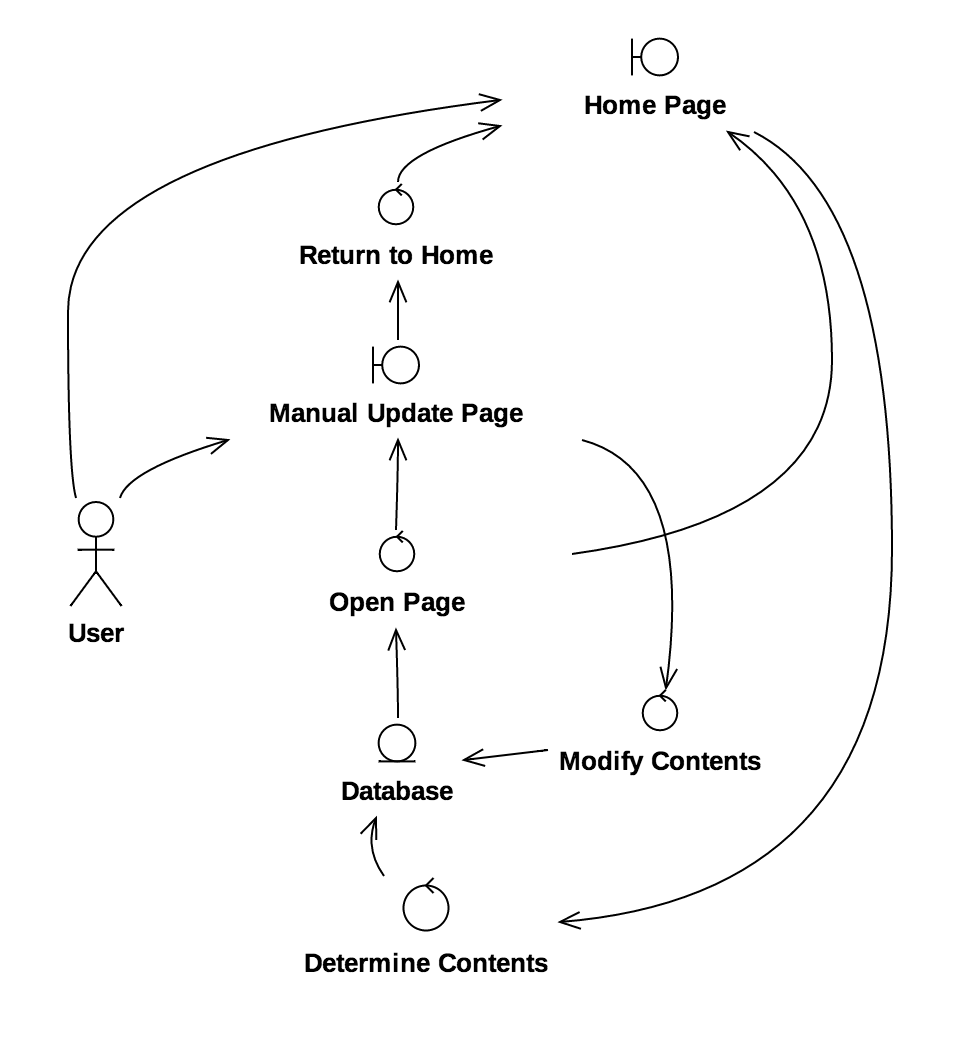
\includegraphics[width=\textwidth]{manualup.png}
			\caption{ Update}
		\end{figure}
	\subsection{Recommend Temperature}
		\subsubsection{Goal:} Recommends optimal fridge temperature based on current items in fridge
		\subsubsection{Input:} Fridge inventory
		\subsubsection{Output:} Optimal Temperature 
		\subsubsection{Main Scenario:} User wishes to reduce energy usage by increasing fridge temperature 
		\subsubsection{Pre-Condition:} Application is running on server, there is at least one item in the fridge inventory, user updates contents
		\subsubsection{Steps:} 
		\begin{enumerate}
			\item Determine items in fridge
			\item Calculate optimal temperature for inventory
			\item From QR code, UPC information is gathered
			\item Display optimal temperature
		\end{enumerate}
		\subsubsection{Representation:} See Figure~\thesubsection
		\begin{figure}[p]
			\centering
			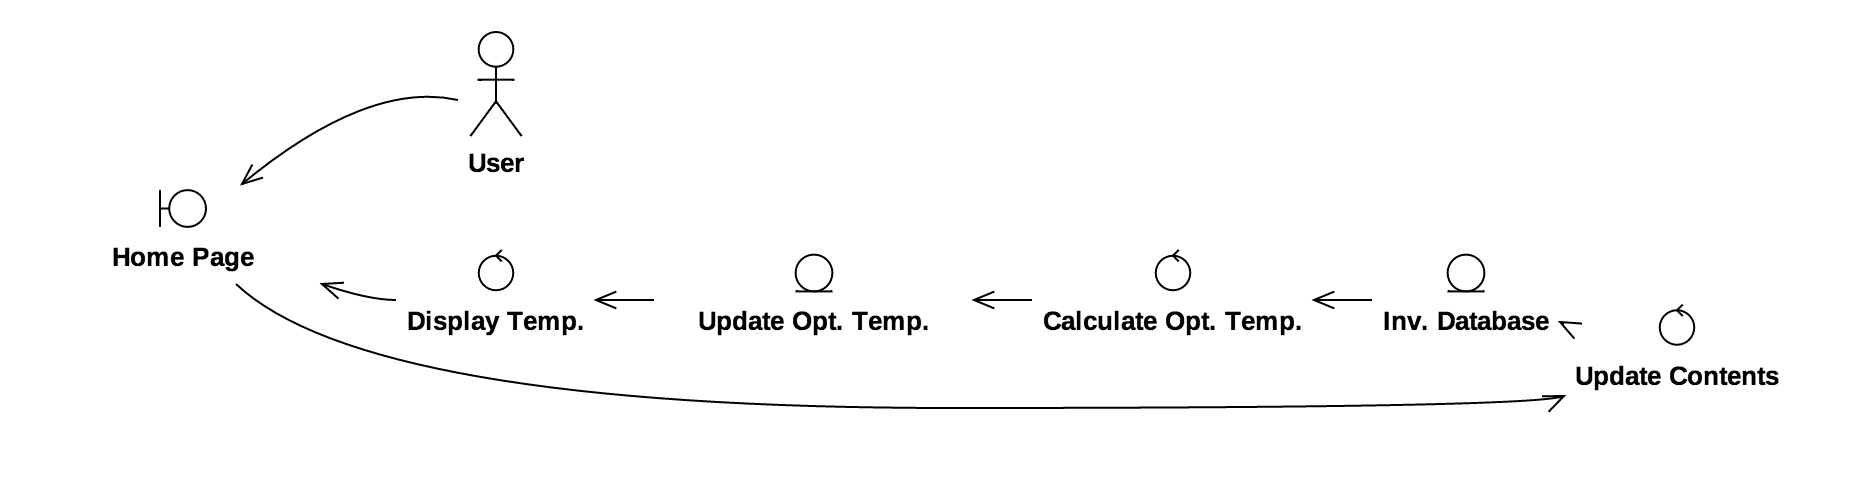
\includegraphics[width=\textwidth]{temp.png}
			\caption{Recommend Temperature}
		\end{figure}
	\subsection{Estimate Waste}
		\subsubsection{Goal:} Estimates food waste due to spoilage
		\subsubsection{Input:} Expired food item 
		\subsubsection{Output:} Amount of food wasted (normalized)
		\subsubsection{Main Scenario:} User wishes to know the amount of food wasted due to spoilage
		\subsubsection{Pre-Condition:} User is logged, food item has expired
		\subsubsection{Steps:} 
		\begin{enumerate}
			\item Query inventory for expired food
			\item Log Expired Food items
			\item Assign value to expired food items
			\item Display value on homepage
		\end{enumerate}
		\subsubsection{Representation:} See Figure~\thesubsection
		\begin{figure}[p]
			\centering
			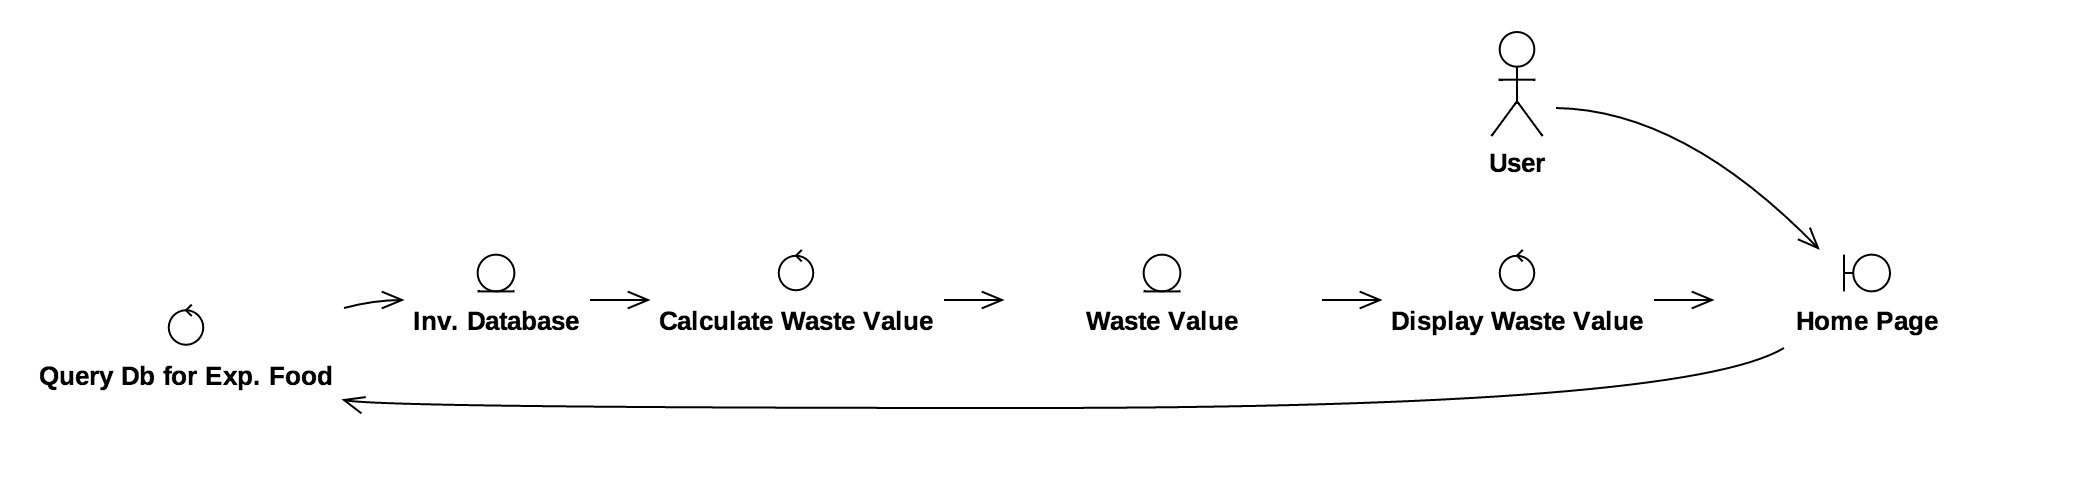
\includegraphics[width=\textwidth]{waste.png}
			\caption{Estimate Waste}
		\end{figure}

	\subsection{Create Shopping List}
		\subsubsection{Goal:} Creates shopping list for user based on recipe requirements and current food in inventory
		\subsubsection{Input:} Recipes, inventory
		\subsubsection{Output:} Shopping list
		\subsubsection{Main Scenario:} User wants to have a shopping list with the items needed for certain recipes, with items already in the inventory not included. 
		\subsubsection{Pre-Condition:} User logged in, recipe page displayed
		\subsubsection{Steps:} 
		\begin{enumerate}
			\item User adds recipe to meal plan
			\item Determine ingredients for recipe
			\item Determine if ingredients are already in inventory
			\item Update Required ingredients list
			\item Add items to shopping list
			\item User opens Shopping List Page
			\item Display shopping list
			\item Print Shopping List
		\end{enumerate}
		\subsubsection{Post-Condition:} Confirm Print
		\subsubsection{Representation:} See Figure~\thesubsection
		\begin{figure}[p]
			\centering
			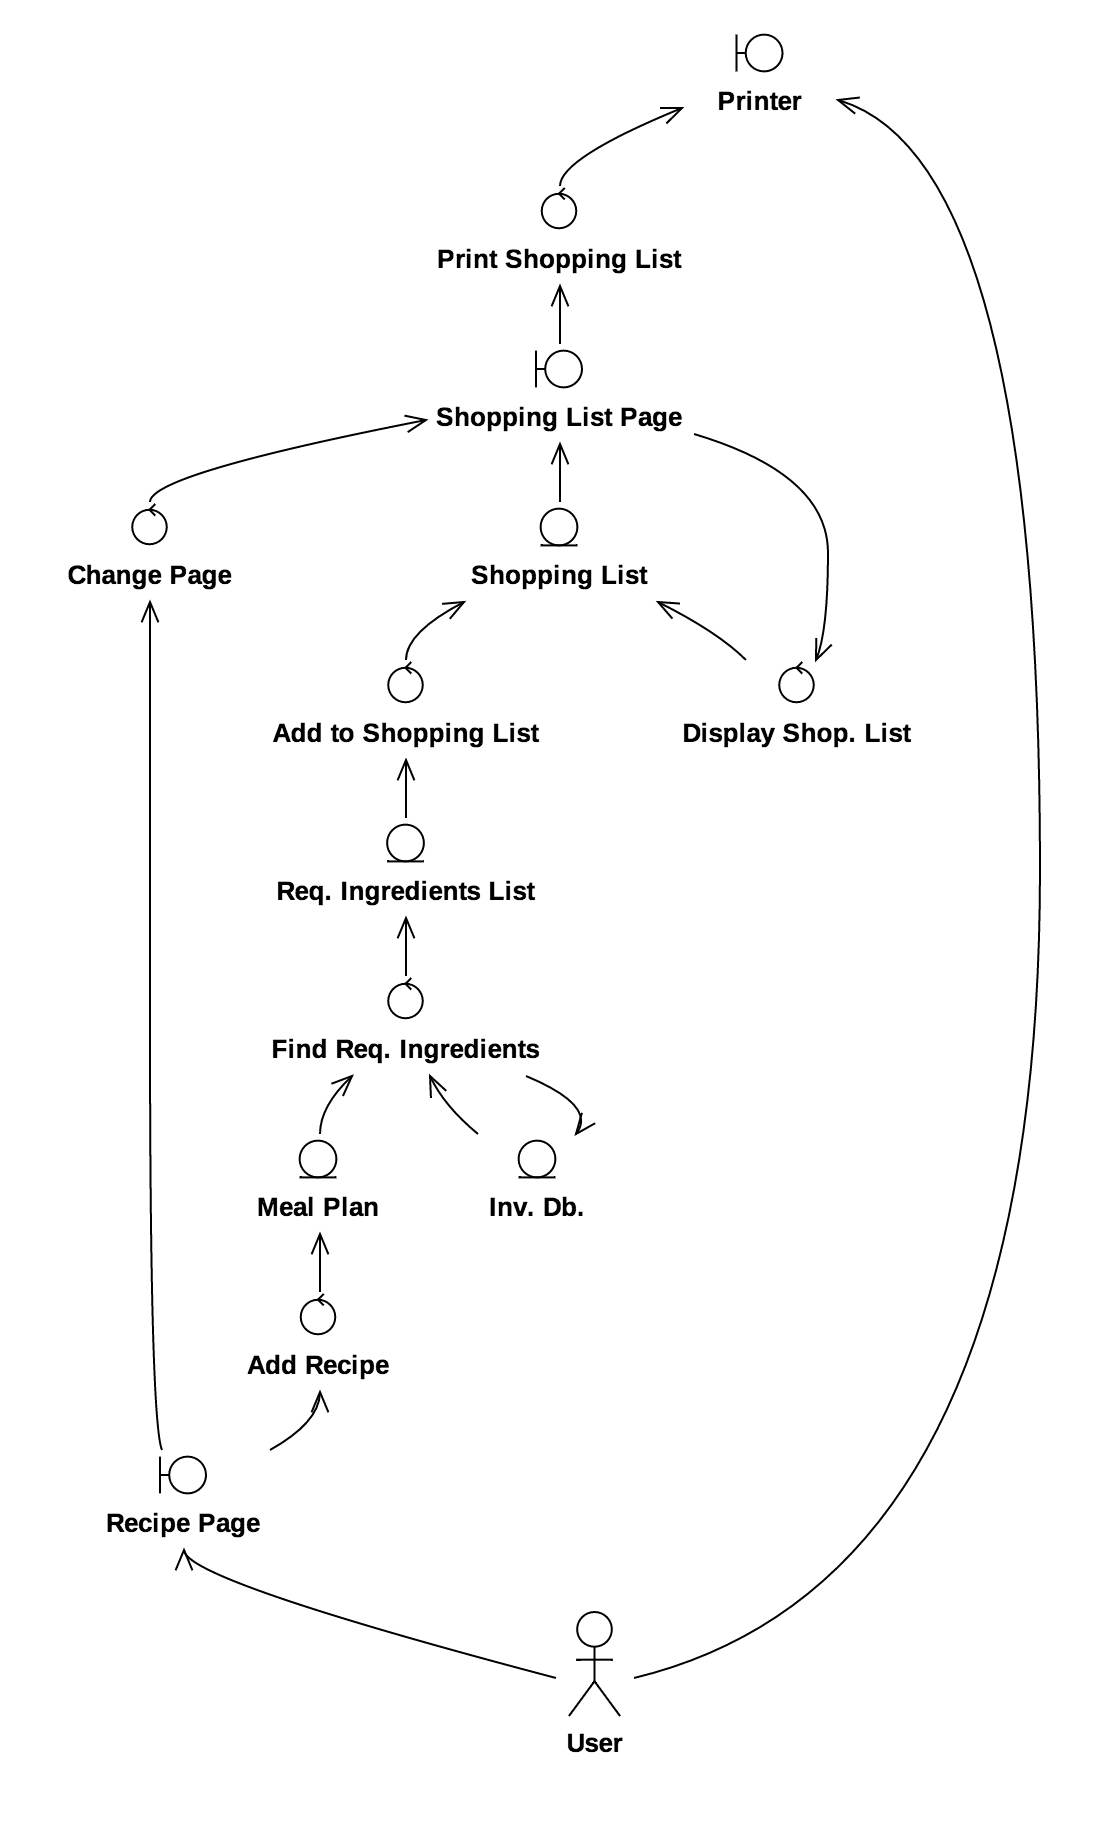
\includegraphics[width=0.5\textwidth]{shopping.png}
			\caption{Create Shopping List}
		\end{figure}


\section{Nonfunctional Requirements} 


\subsection{Performance Requirements}
To ensure that no errors, bugs pop up when user tries to access the software product. Interface between Pillar and Smart fridge must be good so that user does not notify any issues.

\subsection{Safety Requirements}
Safety is a crucial requirement for this system because different users have different nutritional requirements and needs and due importance has to be given to allergies to various food products while generating a personalized food plan.

\subsection{Security Requirements}
Security is also an important aspect as a user’s nutritional plans are confidential in nature. Therefore, measures must be taken to protect the user from nonconsensual leaks of information to 3rd parties (e.g. creators of geared ads). 

\subsection{Software Quality Attributes}
The designed software will be adaptable to any environment, reliable to all users, flexible for different inventories, portable to several devices, and accessible regardless of platform. 


\pagebreak


\end{document}